\section{Regulation}

\begin{multicols}{2}


\section*{Temperature Regulation}


\subsection{Cooling by Sweat}

\begin{center}
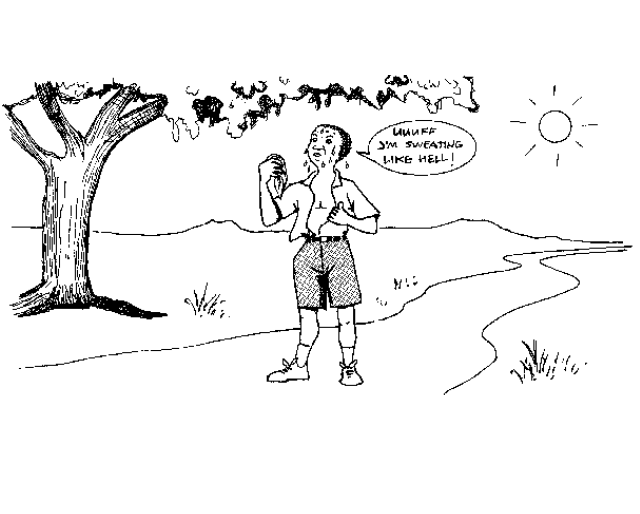
\includegraphics[width=0.49\textwidth]{./img/source/sweating.png}
\end{center}

\begin{description*}
%\item[Subtopic:]{}
%\item[Materials:]{}
%\item[Setup:]{}
\item[Procedure:]{Walk around or do exercise on a hot day.}
%\item[Hazards:]{}
%\item[Questions:]{}
%\item[Observations:]{}
\item[Theory:]{To regulate temperature, our bodies produce sweat. Water droplets on our skin require energy to evaporate, which cools our bodies.}
%\item[Applications:]{}
%\item[Notes:]{}
\end{description*}

\subsection{Evaporation and Cooling}

\begin{center}
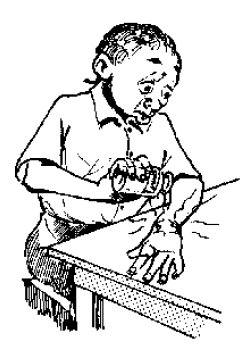
\includegraphics[width=0.3\textwidth]{./img/source/evap-cooling.png}
\end{center}

\begin{description*}
%\item[Subtopic:]{}
\item[Materials:]{Petrol/spirit (e.g. Konyagi)}
%\item[Setup:]{}
\item[Procedure:]{Pour some petrol or spirit on the back of your hand.}
%\item[Hazards:]{}
%\item[Questions:]{}
%\item[Observations:]{}
\item[Theory:]{The back of the hand feels cold, because evaporation of the spirit needs energy which it absorbs from the skin.}
\item[Applications:]{When you go swimming and come out of the water, you feel cold because evaporation of water from your body absorbs heat from your skin. This is also why the body produces sweat in order to cool down.}
%\item[Notes:]{}
\end{description*}


%==================================================================================================%


\end{multicols}

\pagebreak